%-------------------------------------------------------------------------------
\section{Introduction}\label{sec:introduction}
%-------------------------------------------------------------------------------
This document is intended to be a user documentation/manual of the code
\mf{} developed in the framework of the Austrian ESO In-Kind project
SM-03 as described in the corresponding Detailed Specification Document
\cite{SM03DS}.

\mf{} aims at fitting tropospheric/stratospheric telluric features and
deriving correction functions for the removal of these features from spectra of
astronomical targets. The development of the \ac{CPL} workflows is based on an
\ac{IDL} prototype code by A.~Smette (ESO). A preceding version of the code was
developed in the framework of the Austrian ESO In-Kind DR06 project (see
\cite{DR06UM}). \mf{} is also available via a Reflex workflow
with a graphical user interface. A separate document describes this option
(\cite{MFGUI}).

This document is organised as follows: Section~\ref{sec:overview} gives a
brief overview of the project and the incorporated algorithms.
Section~\ref{sec:installation} provides information on the installation
procedures. Section~\ref{sec:running} contains a description on how to run the
code, the required input parameter file, and the output files. In
Section~\ref{sec:model} the atmospheric model and its adaptation to the
observed spectrum are described in detail. Finally, the code performance is
evaluated in Section~\ref{sec:evaluation}.

%-------------------------------------------------------------------------------
\section{Overview}\label{sec:overview}
%-------------------------------------------------------------------------------
\subsection{The project}\label{sec:project}
%-------------------------------------------------------------------------------
Ground-based astronomical observations suffer from emission and absorption
processes in the atmosphere, which deteriorate the quality of the obtained
data. At wavelengths longer than $2 - 2.5$\,$\mu$m, where thermal radiation
from molecules in the lower atmosphere dominates, the amount of this disturbing
background radiation can determine whether scientific observations are feasible
at all. For this wavelength regime, it is crucial to be able to estimate the
intensity of the atmospheric emission in advance. Such a prediction requires
good knowledge of the column densities of atmospheric constituents that
significantly contribute to the greenhouse effect. The most important molecules
are water (H$_2$O), carbon dioxide (CO$_2$), methane (CH$_4$), nitrous oxide
(N$_2$O), and ozone (O$_3$). In particular, a good knowledge of the water
abundance, \ie\ air humidity, is essential, since H$_2$O is the main
contributor to the IR atmospheric spectra. Moreover, it is much more variable
than the other important species. Due to the variability of molecular
abundances, the removal of telluric absorption features from astronomical
spectra depends on observations of telluric standard stars with relatively
smooth continua at similar time and airmass as the scientific target. Even if
those observations are available, the telluric absorption correction becomes
tricky in the near- and mid-IR, where wavelength regions with negligible
atmospheric absorptions are hardly present. In this case, a reliable
determination of the shape of the unabsorbed continuum is very difficult if
an interpolation approach is used. Therefore, a realistic model of the
atmospheric absorption for given observing conditions would make the telluric
absorption correction more reliable and could reduce the number of required
observations of telluric standard stars.

For a periodic monitoring of the abundances of crucial atmospheric constituents
as well as a high-quality correction of telluric absorption features in
astronomical spectra a fast, user-friendly, and reliable software tool is
needed. This project aims at providing such a tool. Thanks to the advances made
in modelling the Earth's atmosphere, it is possible to compute realistic
atmospheric emission and absorption spectra. Such model spectra can be fitted
to observed atmospheric spectra with relative deviations of a few percent only.
The code \mf{} represents such a fitting tool for a reliable
derivation of atmospheric transmission functions and molecular abundances. The
incorporated model spectra are generated by the radiative transfer code
\ac{LBLRTM} \cite{LBLRTM}. The basic input for the radiative transfer code is
an atmospheric profile, which is created from a standard atmosphere (containing
information on height, pressure, temperature, and chemical composition for
general tropical environments up to 120\,km), modelled meteorological \ac{GDAS}
data (containing pressure, temperature, and relative humidity for the region of
the observing site for elevations up to $\approx 25$\,km), and on-site
meteorological measurements by the \ac{EMM}. Using iterative techniques, the
input atmospheric profile is varied to obtain a model spectrum that well fits
the scientific input spectrum (see Section~\ref{sec:algorithm}). In this
process, it is also necessary to optimise the scaling, wavelength grid, and
resolution of the model. For computing radiance spectra reliably, grey body
radiation from the telescope itself has to be taken into account as well.

The resulting software product might be made accessible to the scientific
community. Once adopted by astronomers for atmospheric monitoring purposes, the
efficiency of astronomical instruments working in the thermal IR such as
CRIRES or VISIR could be significantly improved. Since strong molecular
absorption affects all observable wavelength regimes except for the visual,
many ESO instruments could benefit from an improved correction of telluric
features in spectra of astronomical targets. In this document, we will
demonstrate the performance of the code by using CRIRES and X-Shooter spectra
of bright sources and VISIR sky radiance spectra (see
Section~\ref{sec:evaluation}). The test spectra fulfil the minimum calibration
criterion, \ie, they are wavelength-calibrated one-dimensional (1D) spectra
provided as ASCII tables, FITS tables, or FITS images. See section
\ref{sec:inputspec} for more information about the format of the Molecfit input
files.

The C code \mf{} relies on third-party code (see
Section~\ref{sec:requirements}):
\begin{itemize}
    \item C version of the least-squares fitting library {\tt mpfit} by
          C.~Markwardt \cite{CMPFIT} based on the FORTRAN fitting routine
          MINPACK-1 by Mor\'e et al. \cite{MOR80}
    \item The radiative transfer code \lblrtmv. This publicly
          available software is developed within the Radiative Transfer Working
          Group of the \ac{AER}; see also Clough et al. \cite{CLO05},
          \cite{AER}, and \cite{LBLRTM}) for more details. It can handle all
          molecules incorporated in a line parameter database, \eg\ \ac{HITRAN}
          \cite{HITRAN}, and offers a wide range of possibilities to adjust
          input parameters. An additional part of this software is the
          \ac{LNFL}, which provides the required line information on the basis
          of the line parameter database.
    \item A line database of molecular parameters: Currently, the line
          parameter list \aervs{} delivered with the \lblrtmv{}
          package is included in the \mf{} package. This line
          parameter list is build from \ac{HITRAN} 2008 \cite{HITRAN} and
          contains some updates (see \cite{LBLRTM} for more details).
    \item An atmospheric profile valid for the time of observation: The profile
          is created from standard atmospheric profiles, on-site measurements
          by the \ac{EMM} \cite{meteomonitor}, and \ac{GDAS} data (a product of
          the \ac{NCEP} model, created by the \ac{ARL} of the \ac{NOAA}, see
          \cite{AER}, \cite{NOAA}, \cite{GDAS}). Such atmospheric profiles
          contain pressure, temperature, and humidity for a number of layers of
          the atmosphere, at any point on Earth for all recent dates (going
          back to December 2004), on a 3h-grid basis.
    \item Perl scripts {\tt get\_inv.pl} and {\tt get\_grib.pl} from the
          \ac{NCEP} NOMAD server \cite{GRIB} for fast download of \ac{GDAS}
          data in the GRIB2 format.
\end{itemize}

%-------------------------------------------------------------------------------
\subsection{Algorithm}\label{sec:algorithm}
%-------------------------------------------------------------------------------
Schematic graphs of the basic functionality of the software are shown in
Figures~\ref{fig:mf_overview} and ~\ref{fig:mf_detworkflow}, which provide a
general overview of the workflow and the structure of the \mf{}
routine in more detail, respectively.

%-------------------------------------------------------------------------------
\begin{figure}[ht]
\begin{center}
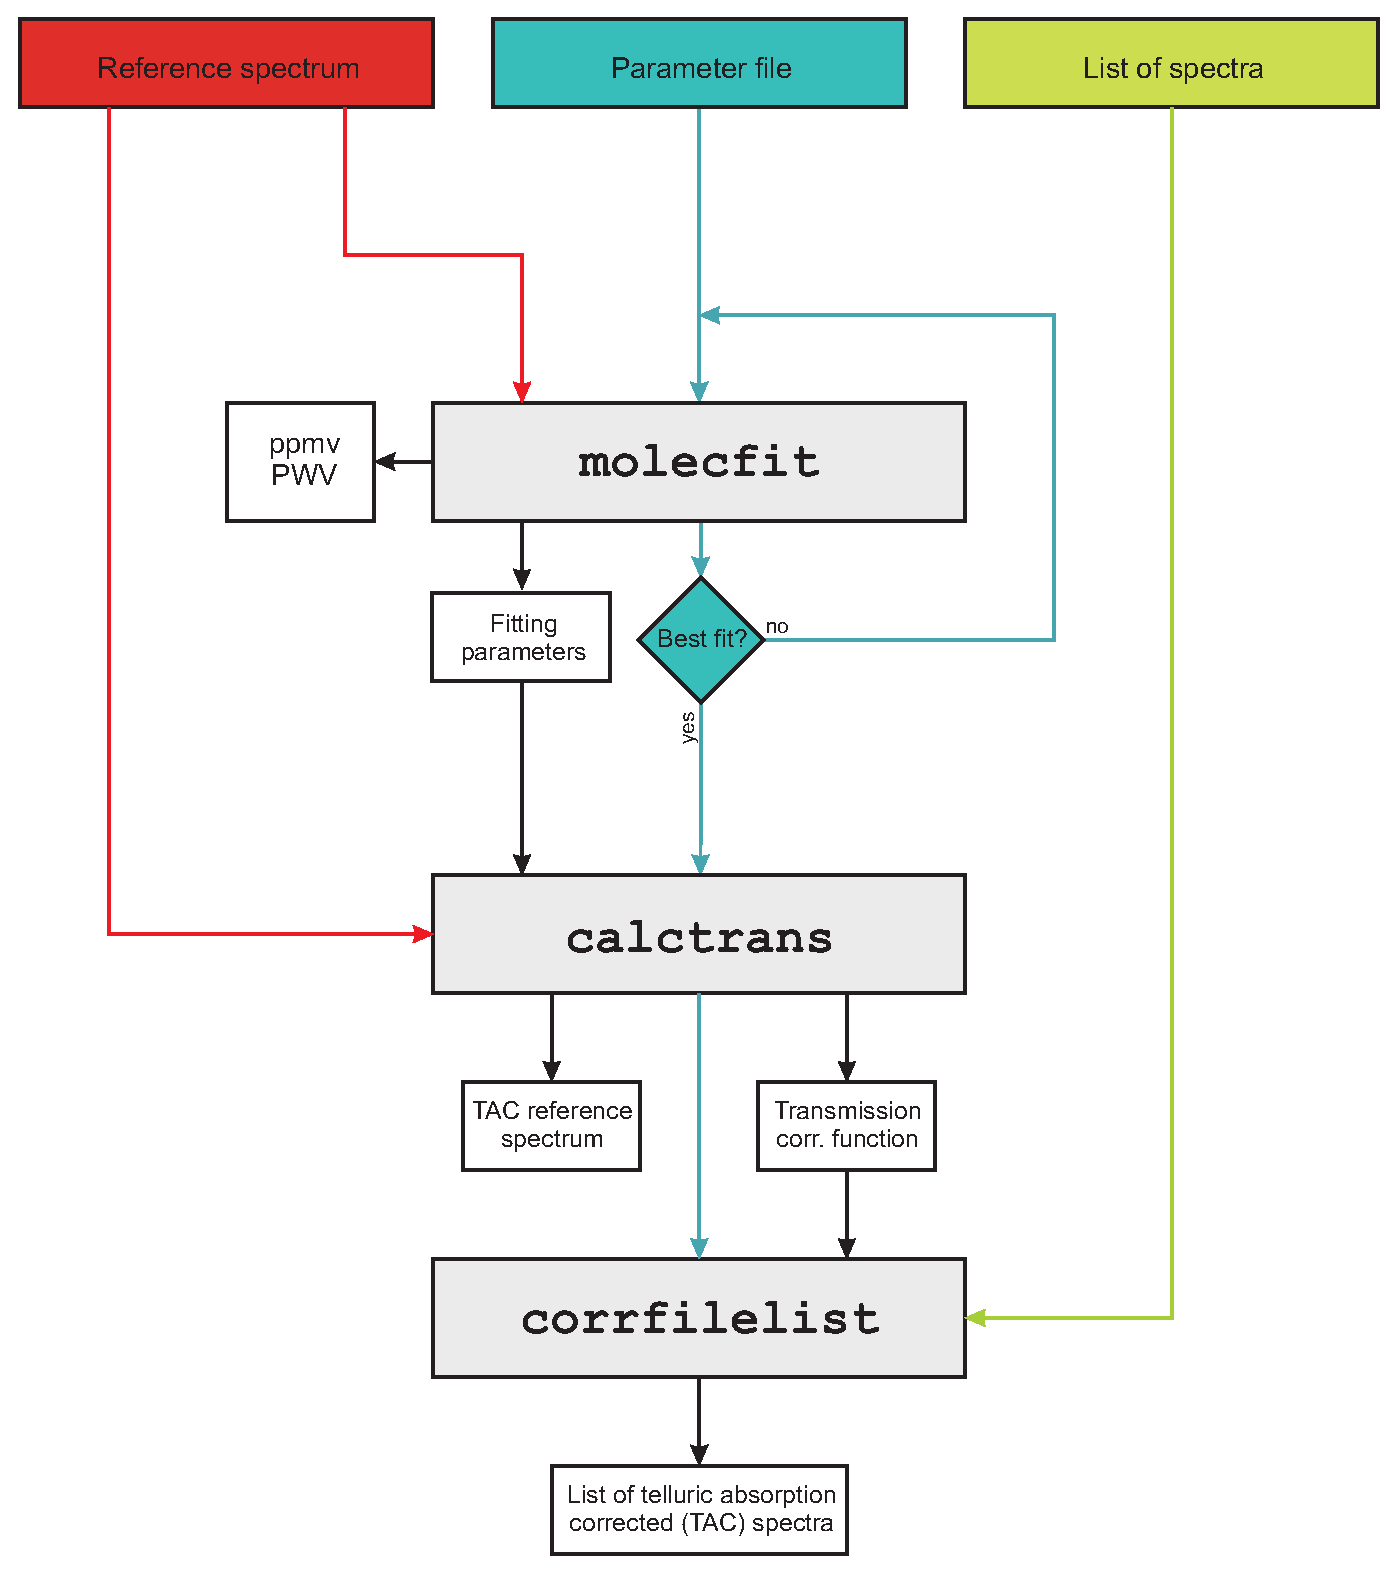
\psfig{file=figures/molecfit_workflow.eps,width=0.9\textwidth}
\caption{Overview of the software workflow. It shows the input and output for
the three executables \mf{}, {\tt calctrans}, and {\tt corrfilelist}
and the connection between these routines.}
\label{fig:mf_overview}
\end{center}
\end{figure}
%-------------------------------------------------------------------------------
%-------------------------------------------------------------------------------
\begin{figure}[ht]
\begin{center}
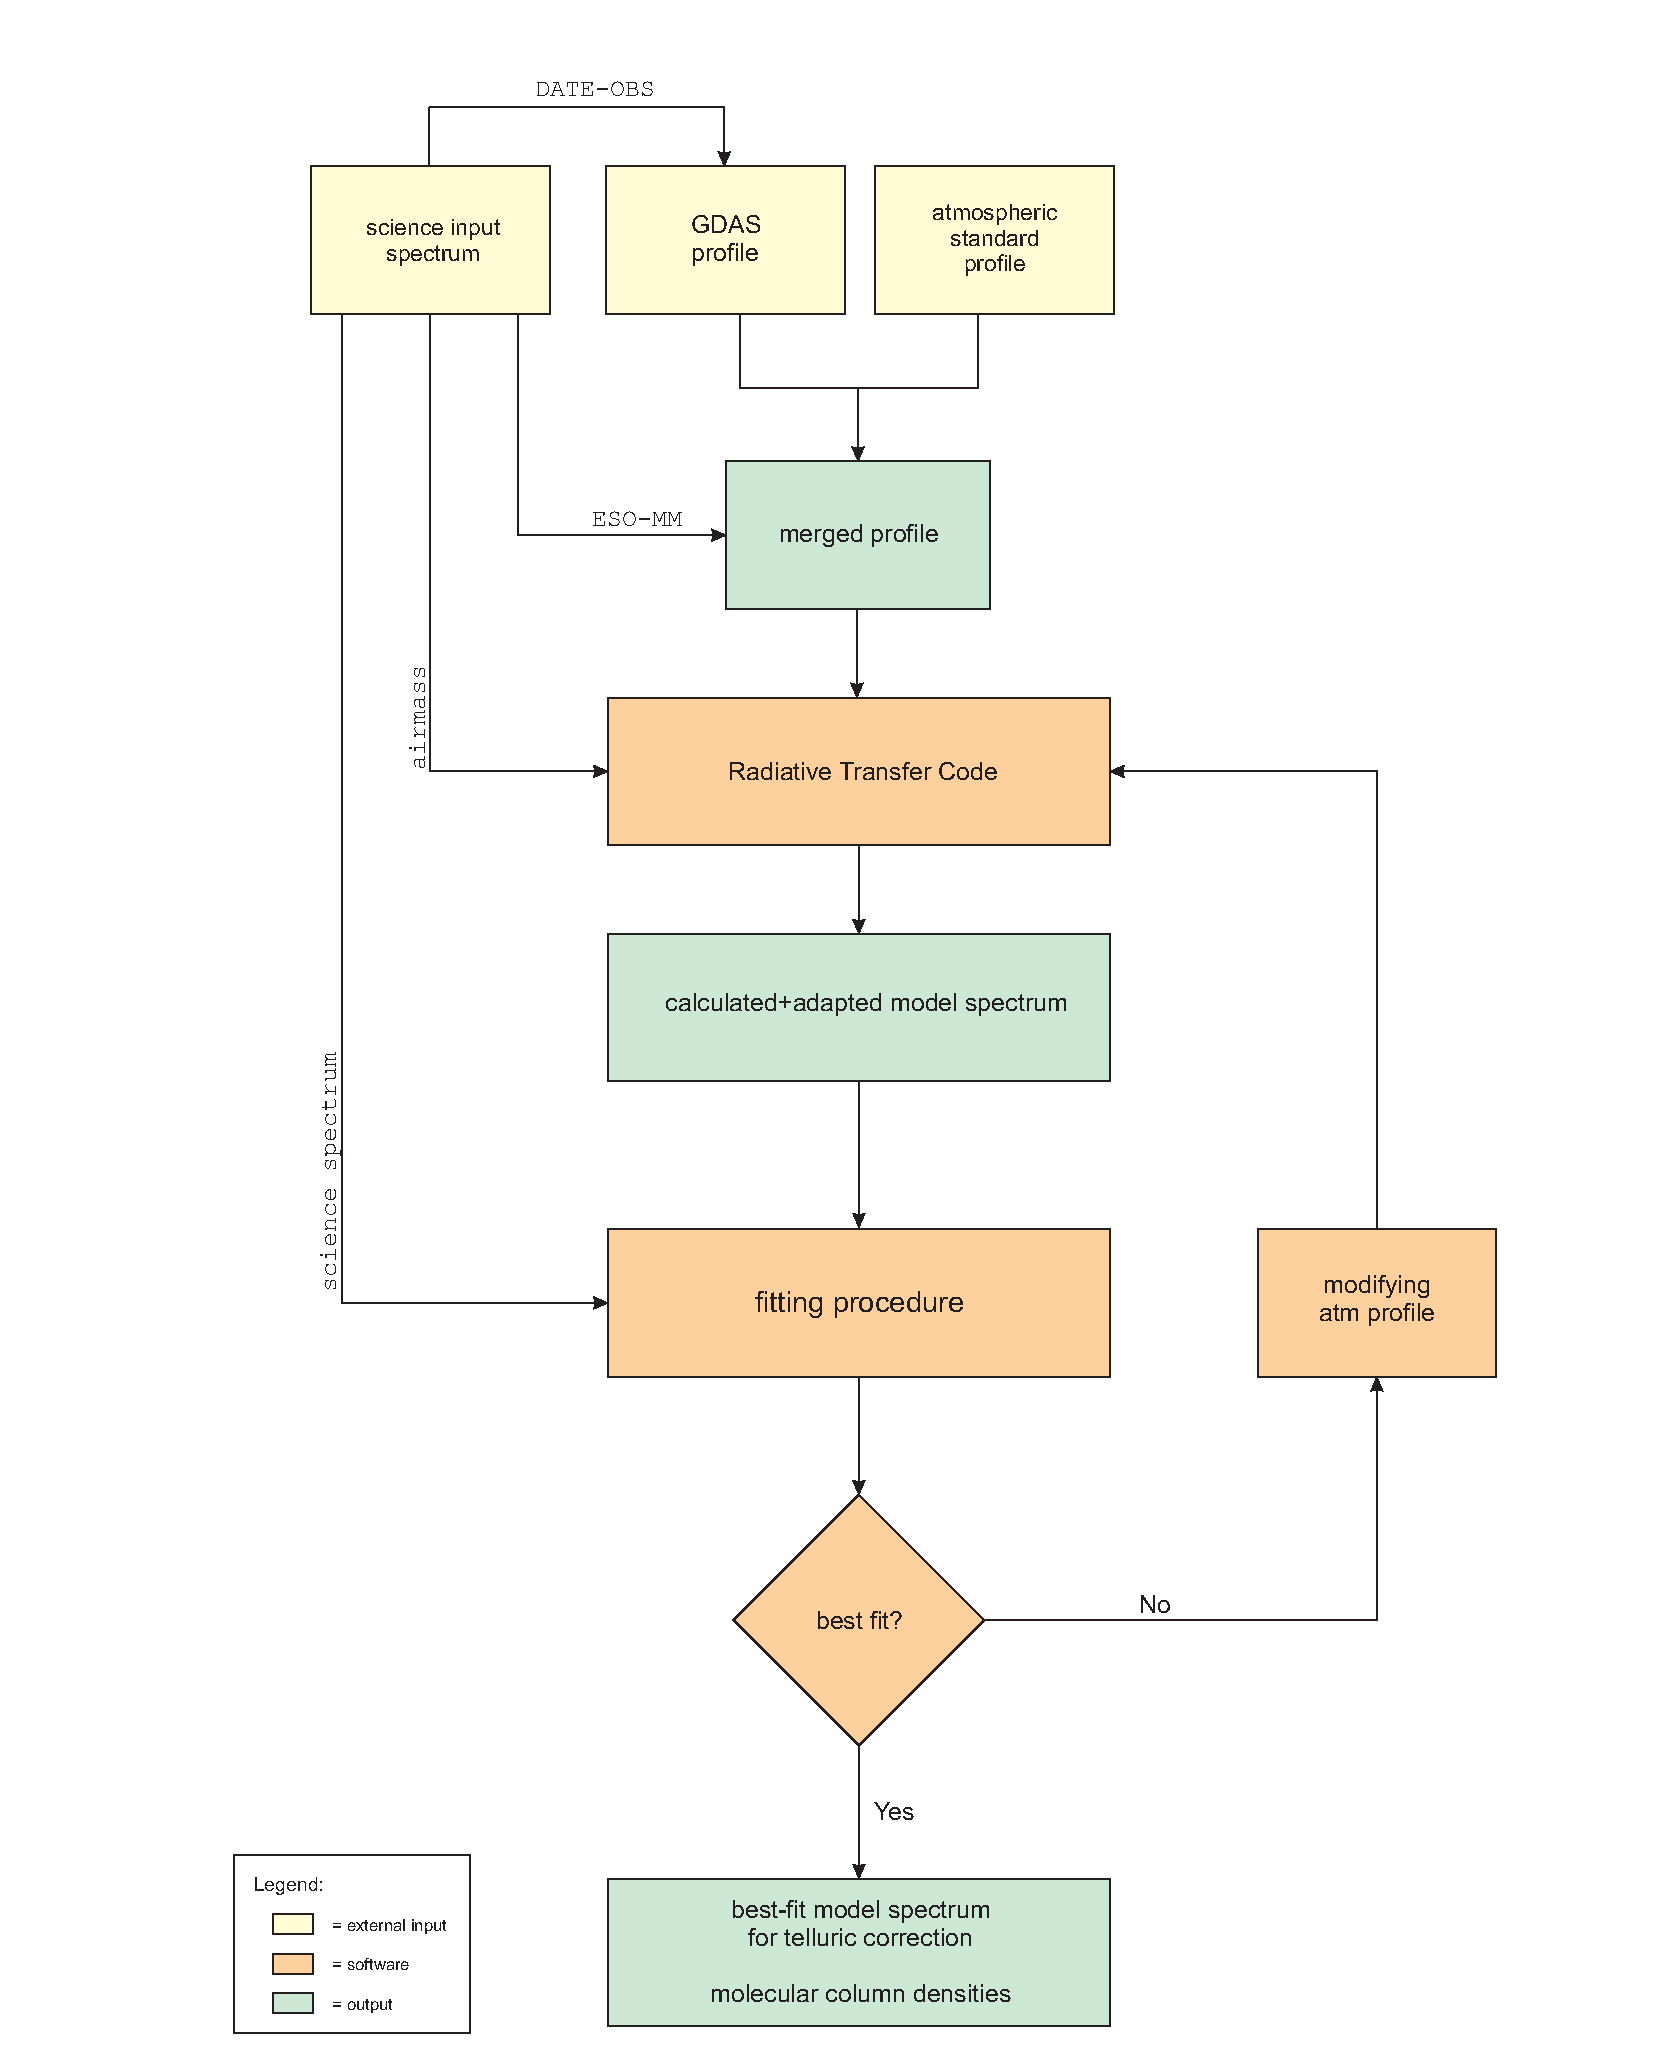
\psfig{file=figures/Overview_SM-03_molecfit.eps,width=0.9\textwidth}
\caption{Workflow of the \mf{} routine.}
\label{fig:mf_detworkflow}
\end{center}
\end{figure}
%-------------------------------------------------------------------------------

First, the code reads the science spectrum from an ASCII table, FITS table, or
FITS image. Furthermore, it reads an ASCII driver file with the user input. If
available, ESO keywords including EMM data are directly taken from a FITS
header. A single atmospheric profile is compiled from data from three sources:
a standard atmospheric profile for a given climate zone, an appropriate
\ac{GDAS} model profile for the time of the observation and the telescope site,
and the corresponding ground-based \ac{EMM} measurements (see
Section~\ref{sec:profiles} for more details). Input for the radiative transfer
model is the resulting merged atmospheric profile (with a possible
pre-selection of relevant molecules) and the target airmass at the time of
observation (see Section~\ref{sec:radcodes}). To match the observed spectrum,
the code adapts the atmospheric spectrum (either transmission or radiation; see
Section~\ref{sec:spectra}) further by flux scaling, wavelength grid correction,
and convolution with a suitable instrumental profile (see
Section~\ref{sec:adaption}). For a radiance spectrum, the contribution of
thermal emission from the telescope is also taken into account (see
Section~\ref{sec:greybody}).

The central component of the algorithm is the comparison/fitting of the
calculated and the input science spectrum by means of {\tt mpfit}
\cite{CMPFIT}. The $\chi^2$ minimisation procedure of this routine is based on
the Levenberg-Marquardt technique (see Mor\'e et al. \cite{MOR80}), an
iterative search algorithm characterised by gradient-controlled jumps in
parameter space. Since this technique is prone to finding local minima,
reasonable starting values and constraints for the fit parameters are required.
{\tt mpfit} checks whether the desired fit quality is reached. If this is not
the case, it changes fit parameters in an appropriate way to search for a better
$\chi^2$. Each function call causes a new calculation of the sky model. For a
change of the molecular abundances, the profiles of molecules can be scaled by
simple factors, which represent a subset of the fit parameters provided to
{\tt mpfit}. The other parameters are coefficients of polynomials for continuum
scaling, coefficients of Chebshev polynomials for the correction of the
wavelength solution, the FWHM of boxcar, Gaussian, and Lorentzian kernels
that are used to build a realistic instrumental profile, and the telescope
emissivity if a radiance spectrum is computed. When a satisfactory fit is
reached after several iterations of the $\chi^2$ minimisation procedure, the
code writes the best-fit spectrum, atmospheric profile, and fit parameters to
output files. The best-fit molecular profiles are integrated to get molecular
columns in ppmv. \mf{} also computes the water vapour content of the
atmosphere in mm. The atmospheric abundances are part of a special output
summary file (see Section~\ref{sec:output}).

The fit parameters are defined in the input driver file (see
Section~\ref{sec:paramfile}). Dynamically setting fit flags to include and
exclude parameters from the fitting procedure allows the code to find a
reasonable solution in a relatively fast and robust way. In detail,
\mf{} follows a plan consisting of six steps by default:
\begin{itemize}
    \item Step 1: scaling of the continuum
    \item Step 2: wavelength and resolution fit
    \item Step 3: rescaling of the continuum
    \item Step 4: fitting of the molecules
    \item Step 5: joint continuum, wavelength, and resolution fit
    \item Step 6: fit of all components (molecules, continuum, wavelength, and
                  resolution)
\end{itemize}
As described in Section~\ref{sec:calling}, it is also possible to focus on the
last step only. Moreover, individual parameters can be fixed for the entire
fitting procedure.

For the telluric absorption correction, the executable {\tt calctrans} has to
be used with the same parameter file as for \mf. {\tt calctrans}
calculates the atmospheric transmission for the full wavelength range of the
input spectrum and corrects this spectrum using this function. These
calculations are separated from the fitting procedure, since the run of a
radiative transfer code for a wide wavelength range is very time consuming.
This is particularly critical if the fit is optimised by several code runs with
different input parameters. For this reason, the fitting procedure should be
performed for several well-defined narrow wavelength ranges that can be
provided by a special ASCII or FITS file (see Section~\ref{sec:paramfile}) if
spectra like those from X-Shooter are processed. Too wide fit ranges are also
not recommended due to the probable failure of the polynomial continuum fit.
The narrow wavelength range of CRIRES allows one to fit the full spectrum at
once. {\tt calctrans} writes a FITS table with the model transmission function,
the telluric absorption corrected spectrum, and a quality flag. Moreover, these
results are provided in the same file format as the input frame, \ie\ ASCII
table, FITS table (with multiple extensions for multiple chips), or 1D FITS
image (with possible extensions for error and quality). For the latter case,
two FITS images are written: one for the correction function and one for the
corrected spectrum (see Section~\ref{sec:output}).

Alternatively, two seperate executables {\tt calctrans\_lblrtm} and 
{\tt calctrans\_convolution} can be used to calculate the atmospheric
transmission and convolve the spectrum respectively.

If other spectra as the fitted one shall be corrected by the same correction
function, an ASCII list of file names can be provided by the input parameter
file (see Section~\ref{sec:paramfile}). The executable {\tt corrfilelist} then
corrects the listed spectra for telluric absorption and saves these spectra in
the same file format as the input files. In addition to the allowed file
formats for \mf, 2D FITS images can be corrected in this way.
